\documentclass[12pt]{article}
\usepackage{graphicx}
\graphicspath{ {./assets/} }
\usepackage[parfill]{parskip}
% \setlength{\parskip}{0pt}
\usepackage[top=0.8in,left=1.6in,right=1.6in]{geometry}

\title{Venus vToken Deposits and Withdrawals \\
    \large Account Behavior in Discrete Time Periods \\~\\
    \large DRAFT}
\author{Sean Hart}

\begin{document}
    \tolerance=5000
    \maketitle

    \begin{abstract}
        \setlength\parskip{1em}
        \noindent Deposits and withdrawals of underlying collateral from vToken contracts in the Venus protocol are key indicators of account behavior because they can indicate investment longevity (accounts and assets that are more likely to deposit long-term). Investment longevity is one important metric to understanding TVL (Total Value Locked) stability of the Venus protocol.

        \noindent In this analysis, deposits and withdrawals will be primarily analyzed over monthly time periods to distinguish the behavior of different accounts over a moderate time range.
    \end{abstract}

    \section*{Introduction}
        The Venus lending and borrowing features function by wrapping deposited collateral in "vTokens" to represent locked assets. For example, deposited USDC tokens are represented by Venus minting vUSDC tokens and adding the appropriate balance of vUSDC to the address that deposited the USDC. Deposits and withdrawals can be tracked by aggregating collateral token transfers to and from vToken contracts. The net flow of funds to and from vToken contracts can be used to summarize the behavior of a specific account in a particular time period. This historic account behavior can be used to help predict future behavior.

    \section*{Common Terms}
        \begin{itemize}{}{}
            \item Account / User: A specific address interacting with the Venus protocol
            \item Collateral Token: The specific asset type deposited into the Venus protocol and represented by a vToken (e.g. USDC)
            \item Deposit: The transfer of a Collateral Token into the Venus protocol
            \item Investment Longevity: Depositing assets in the Venus protocol for long periods of time (relative to other crypto investments)
            \item Net Fund Flow / Net Flow of Funds: Collateral Token deposits minus withdrawals over a specific time period
            \item vToken: A Venus-controlled BEP-20 contract that tracks a specific asset type deposited in the Venus protocol (e.g. vUSDC for the USDC asset)
            \item Withdrawal: The transfer of a Collateral Token out of the Venus protocol
        \end{itemize}

    \section*{Six Month Account Distribution}
        Before segmenting account fund flows into monthly time periods, we can consider six months of activity to understand general account behavior patterns.

        We will use the most commonly used asset on Venus to demonstrate.
        \begin{figure}[h]
            \caption{2021 asset transfer counts between Collateral Tokens and vTokens \label{overflow}}
            \centering
            \hspace*{0in}
            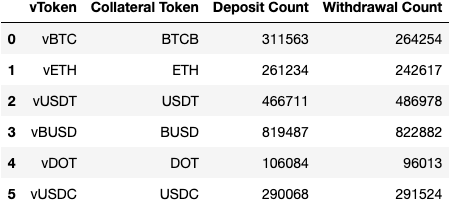
\includegraphics[width=0.5\paperwidth]{transfer-count.png}
        \end{figure}

        Although BUSD is not the asset with the most collateral value on Venus, it is clearly utilized as collateral in the most transactions. It will be a good demonstration of account fund flows for assets.
        \clearpage

        \begin{figure}[h]
            \caption{BUSD Net Fund Flows in/out of vBUSD by Account (H2 2021) \label{overflow}}
            \centering
            \hspace*{-1in}
            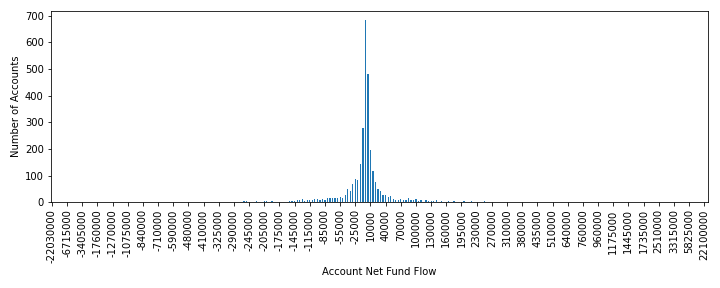
\includegraphics[width=0.8\paperwidth]{net-fundflow-accountdist-busd-H2-2021.png}
        \end{figure}

        We can see from the graph\footnote{https://dune.xyz/queries/326955} that distribution of fund flows has a high kurtosis, meaning that the vast majority of accounts have a low net fund flow, while few accounts have extremely unbalanced fund flows (either deposits or withdrawals). A low net fund flow means that most accounts either do not deposit or withdraw much, or they deposit and withdraw nearly equal amounts.

        This analysis draft will only analyze net fund flows. Additional analysis is needed to analyze the quantity of fund flows relative to the net fund flow per account.

    \section*{Monthly Analysis (Q4 2021)}
        Now we will analyze each asset for the three month period during the fourth quarter of 2021. This segmentation of the data will help us understand behavior differences between asset types and different recent months.
        \clearpage

        \subsection*{vBTC}
            For vBTC, we will consider the BSC BTCB token's deposits and withdrawals\footnote{https://dune.xyz/queries/326786}.
            % \clearpage

            \begin{figure}[h]
                \caption{BTCB Net Fund Flows in/out of vBTC by Account (10-2021) \label{overflow}}
                \centering
                \hspace*{-1in}
                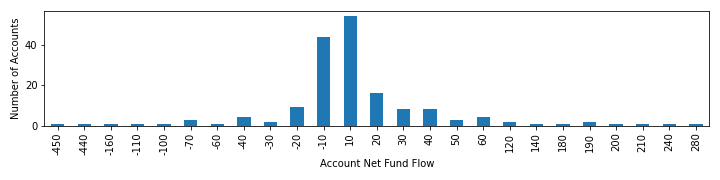
\includegraphics[width=0.8\paperwidth]{net-fundflow-accountdist-vBTC-10-2021.png}
                % \vspace{<whatever>}

                \caption{BTCB Net Fund Flows in/out of vBTC by Account (11-2021) \label{overflow}}
                \centering
                \hspace*{-1in}
                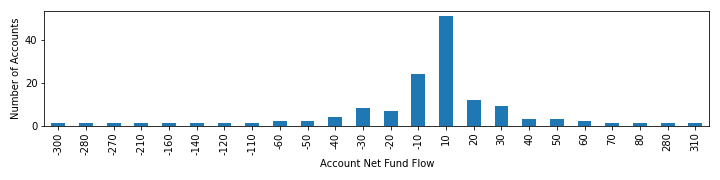
\includegraphics[width=0.8\paperwidth]{net-fundflow-accountdist-vBTC-11-2021.png}

                \caption{BTCB Net Fund Flows in/out of vBTC by Account (12-2021) \label{overflow}}
                \centering
                \hspace*{-1in}
                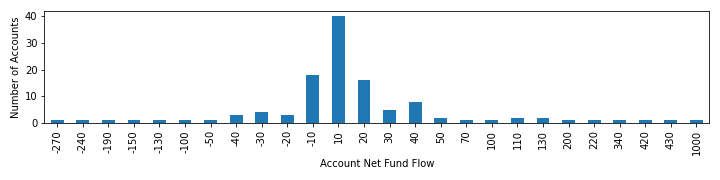
\includegraphics[width=0.8\paperwidth]{net-fundflow-accountdist-vBTC-12-2021.png}
            \end{figure}

            Bitcoin is much more valuable per token than other assets, so here we see that the raw net fund flow figures are low. We also see the distribution slightly skewed toward withdrawals in October and November.
            \clearpage

        \subsection*{vETH}
            For vETH, we will consider the BSC ETH-pegged token's deposits and withdrawals\footnote{https://dune.xyz/queries/326631}.
            \begin{figure}[h]
                \caption{ETH Net Fund Flows in/out of vETH by Account (10-2021) \label{overflow}}
                \centering
                \hspace*{-1in}
                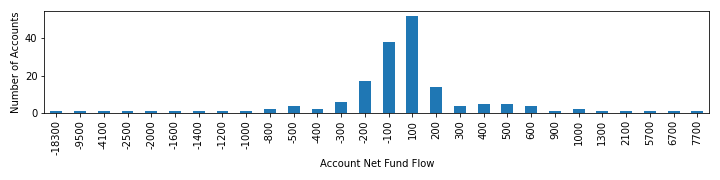
\includegraphics[width=0.8\paperwidth]{net-fundflow-accountdist-vETH-10-2021.png}

                \caption{ETH Net Fund Flows in/out of vETH by Account (11-2021) \label{overflow}}
                \centering
                \hspace*{-1in}
                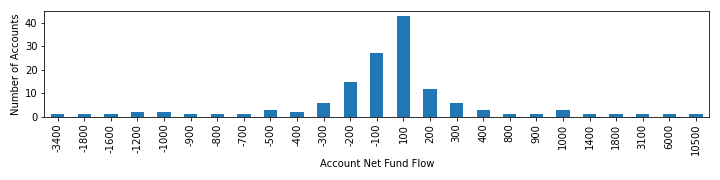
\includegraphics[width=0.8\paperwidth]{net-fundflow-accountdist-vETH-11-2021.png}

                \caption{ETH Net Fund Flows in/out of vETH by Account (12-2021) \label{overflow}}
                \centering
                \hspace*{-1in}
                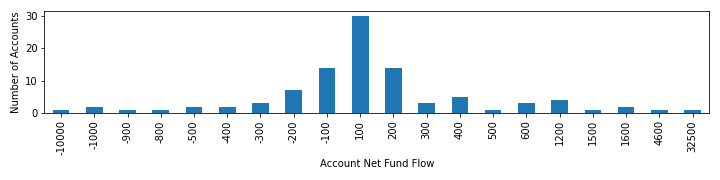
\includegraphics[width=0.8\paperwidth]{net-fundflow-accountdist-vETH-12-2021.png}
            \end{figure}

            Ethereum also has a distribution skewed toward withdrawals in October and November.
            \clearpage
        
        \subsection*{vUSDT}
            For vUSDT, we will consider the BSC USDT token's deposits and withdrawals\footnote{https://dune.xyz/queries/326728}.
            \begin{figure}[h]
                \caption{USDT Net Fund Flows in/out of vUSDT by Account (10-2021) \label{overflow}}
                \centering
                \hspace*{-1in}
                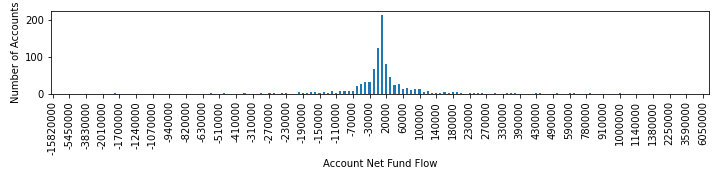
\includegraphics[width=0.8\paperwidth]{net-fundflow-accountdist-vUSDT-10-2021.png}

                \caption{USDT Net Fund Flows in/out of vUSDT by Account (11-2021) \label{overflow}}
                \centering
                \hspace*{-1in}
                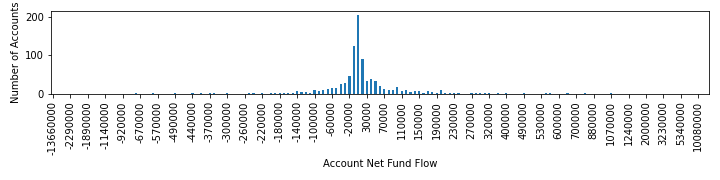
\includegraphics[width=0.8\paperwidth]{net-fundflow-accountdist-vUSDT-11-2021.png}

                \caption{USDT Net Fund Flows in/out of vUSDT by Account (12-2021) \label{overflow}}
                \centering
                \hspace*{-1in}
                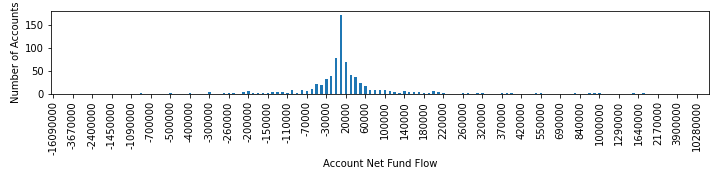
\includegraphics[width=0.8\paperwidth]{net-fundflow-accountdist-vUSDT-12-2021.png}
            \end{figure}

            USDT is a very commonly used asset on the Binance Smart Chain, and it appears to have a fairly even distribution, but with extremely long tails.
            \clearpage

        \subsection*{vBUSD}
            For vBUSD, we will consider the BUSD token's deposits and withdrawals\footnote{https://dune.xyz/queries/326950}.
            \begin{figure}[h]
                \caption{BUSD Net Fund Flows in/out of vBUSD by Account (10-2021) \label{overflow}}
                \centering
                \hspace*{-1in}
                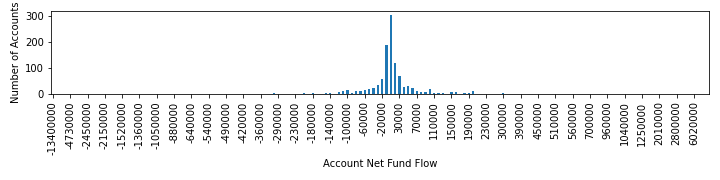
\includegraphics[width=0.8\paperwidth]{net-fundflow-accountdist-vBUSD-10-2021.png}

                \caption{BUSD Net Fund Flows in/out of vBUSD by Account (11-2021) \label{overflow}}
                \centering
                \hspace*{-1in}
                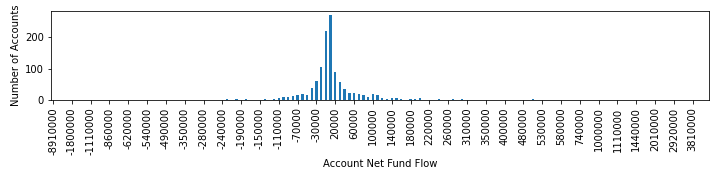
\includegraphics[width=0.8\paperwidth]{net-fundflow-accountdist-vBUSD-11-2021.png}

                \caption{BUSD Net Fund Flows in/out of vBUSD by Account (12-2021) \label{overflow}}
                \centering
                \hspace*{-1in}
                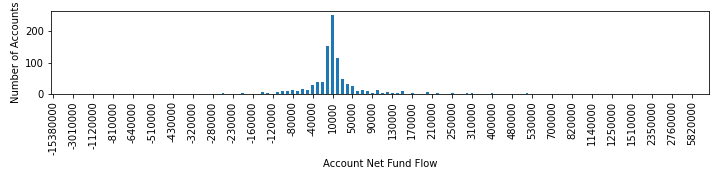
\includegraphics[width=0.8\paperwidth]{net-fundflow-accountdist-vBUSD-12-2021.png}
            \end{figure}

            Binance's USD-pegged token also has a distribution skewed slightly toward withdrawals and extremely long tails, similar to USDT.
            \clearpage

        \subsection*{vDOT}
            For vDOT, we will consider the BSC DOT-pegged token's deposits and withdrawals\footnote{https://dune.xyz/queries/326954}.
            \begin{figure}[h]
                \caption{DOT Net Fund Flows in/out of vDOT by Account (10-2021) \label{overflow}}
                \centering
                \hspace*{-1in}
                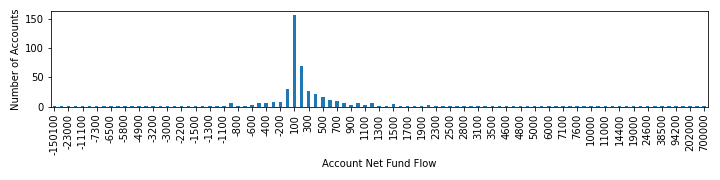
\includegraphics[width=0.8\paperwidth]{net-fundflow-accountdist-vDOT-10-2021.png}

                \caption{DOT Net Fund Flows in/out of vDOT by Account (11-2021) \label{overflow}}
                \centering
                \hspace*{-1in}
                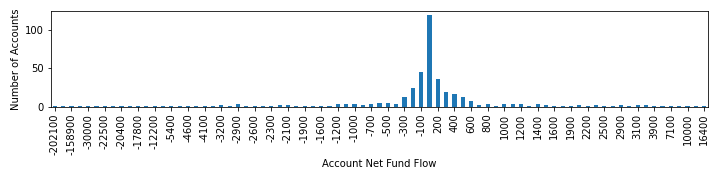
\includegraphics[width=0.8\paperwidth]{net-fundflow-accountdist-vDOT-11-2021.png}

                \caption{DOT Net Fund Flows in/out of vDOT by Account (12-2021) \label{overflow}}
                \centering
                \hspace*{-1in}
                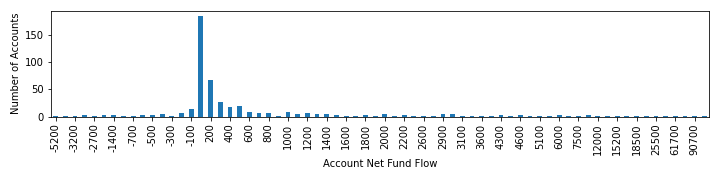
\includegraphics[width=0.8\paperwidth]{net-fundflow-accountdist-vDOT-12-2021.png}
            \end{figure}

            DOT has a distribution skewed toward deposits in December, including high-value deposits. DOT's December deposits deserve additional analysis.
            \clearpage

        \subsection*{vUSDC}
            For vUSDC, we will consider the BSC USDC-pegged token's deposits and withdrawals\footnote{https://dune.xyz/queries/323328}.
            \begin{figure}[h]
                \caption{USDC Net Fund Flows in/out of vUSDC by Account (10-2021) \label{overflow}}
                \centering
                \hspace*{-1in}
                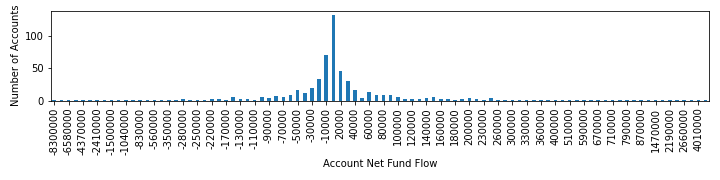
\includegraphics[width=0.8\paperwidth]{net-fundflow-accountdist-vUSDC-10-2021.png}

                \caption{USDC Net Fund Flows in/out of vUSDC by Account (11-2021) \label{overflow}}
                \centering
                \hspace*{-1in}
                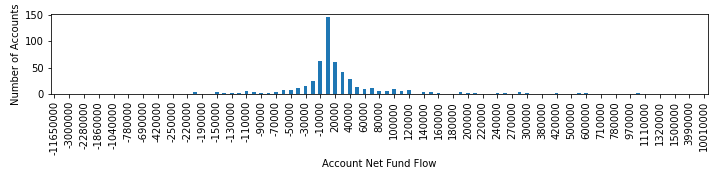
\includegraphics[width=0.8\paperwidth]{net-fundflow-accountdist-vUSDC-11-2021.png}

                \caption{USDC Net Fund Flows in/out of vUSDC by Account (12-2021) \label{overflow}}
                \centering
                \hspace*{-1in}
                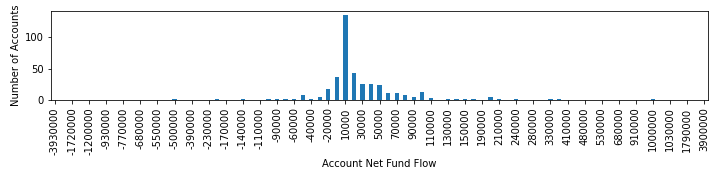
\includegraphics[width=0.8\paperwidth]{net-fundflow-accountdist-vUSDC-12-2021.png}
            \end{figure}

            Similar to other USD-pegged tokens like USDT and BUSD, USDC withdrawal and deposits have extremely long tails.
            \clearpage
        
    \section*{Findings (Preliminary)}
        Initial conclusions from this data include:
        \begin{itemize}{}{}
            \item Most accounts deposit and withdraw similar amounts each month. This likely means short-term investments by these accounts.
            \item USD-pegged tokens (USDT, BUSD, USDC) have extremely long tails, which likely means accounts that use these tokens to deposit or withdraw invest for at least one month. Actual time ranges of these high-value accounts need more analysis.
        \end{itemize}

        These conclusions involve many assumptions. This data requires further analysis to be effective for use in strategic decisions.

\end{document}